\chapter{Concetti essenziali di teoria dei grafi}
\label{chap:cap2}

Le assunzioni secondo cui ogni individuo possa entrare in contatto con chiunque (\emph{mixing omogeneo}) e il numero di interazioni di ciascun soggetto sia confrontabile con quello degli altri non sono realistiche: la probabilità che si verifichi un incontro fra due individui presi a caso è praticamente infinitesima, ma, al contrario, quella che due compartimenti distinti entrino in relazione l'uno con l'altro è senza dubbio finita. Di norma, i contatti fra individui sono limitati ad un numero ristretto di persone (familiari, colleghi, etc), mentre tutto il resto della popolazione viene ignorato; questo li rende particolarmente adatti ad essere rappresentati tramite una rete \cite{Barabasi}. 
%\medskip 
\section{Tipi di grafo}
Andiamo ad introdurre una serie di definizioni che in seguito ci risulteranno utili.
\begin{definizione}[\textit{Grafo}]
Un \emph{grafo} (o una \emph{rete}) è un insieme di elementi detti vertici o \emph{nodi} che possono essere collegati fra loro da segmenti detti archi o \emph{link} \cite{Bickle}.
\end{definizione}
\subsection{Grafi non orientati}
\begin{figure}
		\begin{center}
			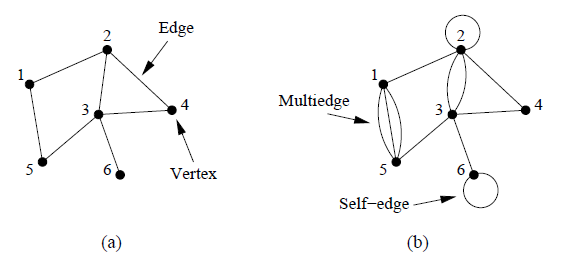
\includegraphics[scale=.8, keepaspectratio]{network_example}
			\caption{(a) Un grafo semplice, cioè privo di loop o link multipli. (b) Un grafo che presenta entrambi \cite{Newman}.}
			\label{fig:net_ex}
		\end{center}
	\end{figure}
	
Consideriamo una rete non orientata - cioè una rete in cui i link possono essere percorsi indistintamente in un verso e nell'altro - con $ n $ vertici, che andiamo ad etichettare da $ 1 $ a $ n $. Se indichiamo con $ \left( i, j \right) $ l'arco fra i nodi $ i $ e $ j $, allora l'intera rete può essere descritta in funzione della
\begin{definizione}[\textit{Matrice di adiacenza I}]
La matrice di adiacenza \textbf{A} relativa ad un grafo semplice è una matrice i cui elementi sono così definiti \cite{Newman}:
\[
A_{ij} \, =
\begin{cases}
1, & \text{se esiste un arco fra $ i $ e $ j $};\\ 
0, & \text{altrimenti}.
\end{cases}
\]
\end{definizione}
Se, ad esempio, prendiamo la rete (a) in \cref{fig:net_ex}, assumerà la seguente forma:
\begin{equation}
A =
\begin{pmatrix}
0 & 1 & 0 & 0 & 1 & 0 \\
1 & 0 & 1 & 1 & 0 & 0 \\
0 & 1 & 0 & 1 & 1 & 1 \\
0 & 1 & 1 & 0 & 0 & 0 \\
1 & 0 & 1 & 0 & 0 & 0 \\
0 & 0 & 1 & 0 & 0 & 0
\end{pmatrix} .
\end{equation}
Possiamo osservare che risulta essere una matrice simmetrica con tutti $ 0 $ sulla diagonale. 
\\Qualora invece ne avessimo sotto esame una più simile alla rete (b) della medesima figura, dovremmo tener conto del fatto che sono presenti link multipli e loop; si stabilisce di assegnare ai primi un numero pari alla loro molteplicità e ai secondi il valore $ 2 $. Ne risulta una matrice, ancora una volta, simmetrica:
\begin{equation}
A =
\begin{pmatrix}
0 & 1 & 0 & 0 & 3 & 0 \\
1 & 2 & 2 & 1 & 0 & 0 \\
0 & 2 & 0 & 1 & 1 & 1 \\
0 & 1 & 1 & 0 & 0 & 0 \\
3 & 0 & 1 & 0 & 0 & 0 \\
0 & 0 & 1 & 0 & 0 & 2
\end{pmatrix} .
\end{equation}

\subsection{Digrafi}
\begin{wrapfigure}{l}{0.4\textwidth}
		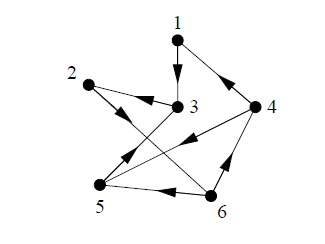
\includegraphics[width=0.38\textwidth]{digraph_example}
		\caption{Un digrafo \cite{Newman}.}
		\label{fig:dig_ex}
\end{wrapfigure}
La questione cambia leggermente se si va a considerare una rete diretta o \emph{digrafo}.
\begin{definizione}[\textit{Digrafo}]
Un \emph{digrafo} è un tipo di grafo in cui ogni arco ha una direzione, punta cioè da un vertice ad un altro \cite{Newman}.
\end{definizione}
Ciò ci porta a rivedere quanto detto per la matrice di adiacenza: affermiamo, quindi, che
\begin{definizione}[\textit{Matrice di adiacenza II}]
La matrice di adiacenza \textbf{A} relativa ad un grafo orientato è una matrice i cui elementi sono così definiti \cite{Newman}:
\[
A_{ij} \, =
\begin{cases}
1, & \text{se esiste un arco da $ j $ a $ i $};\\ 
0, & \text{altrimenti}.
\end{cases}
\]
\end{definizione}

Relativamente alla \cref{fig:dig_ex}, la matrice assumerà, pertanto, la seguente forma: \\
\begin{equation}
A =
\begin{pmatrix}
0 & 0 & 0 & 1 & 0 & 0 \\
0 & 0 & 1 & 0 & 0 & 0 \\
1 & 0 & 0 & 0 & 1 & 0 \\
0 & 0 & 0 & 0 & 0 & 1 \\
0 & 0 & 0 & 1 & 0 & 0 \\
0 & 1 & 0 & 0 & 0 & 0
\end{pmatrix} .
\end{equation}
\subsection{Grafi bipartiti}
Ci soffermiamo poi su un ulteriore tipo di grafo, che ci risulterà più utile in seguito.
\begin{definizione}[\textit{Grafo bipartito}] 
Un grafo si dice \emph{bipartito} se i suoi vertici possono essere suddivisi in due sottoinsiemi X e Y tali che ogni link ha un'estremità in X ed una in Y \cite{Bondy}. 
\end{definizione}
\begin{figure}[h]
	\begin{center}
		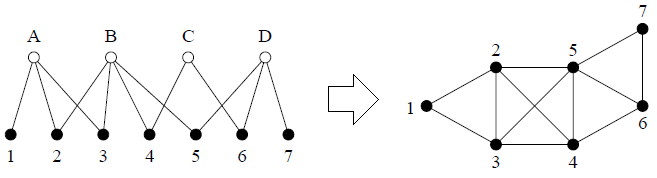
\includegraphics[scale=0.7]{projections2}
		\caption{Passaggio da una rappresentazione tipica di una rete bipartita ad una in cui compaiono solo i vertici \cite{Newman}.}
		\label{fig:proj2}
	\end{center}
\end{figure}

In modo del tutto equivalente a quanto abbiamo già fatto, possiamo andare a definire per un grafo del genere una matrice che lo va a descrivere.
\begin{definizione}[\textit{Matrice di incidenza}]
La matrice di incidenza \textbf{B} è una matrice $ g \times n $, dove $ g $ è il numero di sottoinsiemi e $ n $ quello dei vertici che ne fanno parte, i cui elementi sono definiti come segue \cite{Newman}:
\[
B_{ij} \, =
\begin{cases}
1, & \text{se il vertice $ j $ appartiene al gruppo $ i $ };\\
0, & \text{altrimenti}.
\end{cases}
\]
\end{definizione}

%\begin{wrapfigure}{r}{0.7\textwidth}
%	\begin{center}
%		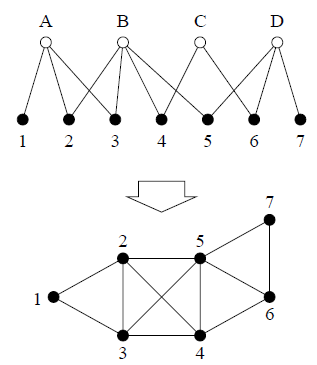
\includegraphics[width=0.35\textwidth]{projections}
%	\end{center}
%	\caption{
%%	In figura si mette in luce il passaggio da una rappresentazione tipica di una rete bipartito ad una in cui compaiono solo i vertici. 
%	\cite{Newman}}
%	\label{fig:projs}
%\end{wrapfigure}
Uno dei pregi di una rete bipartita è quello di consentire in modo fluido il passaggio da una rappresentazione in cui compaiono sia vertici che gruppi ad una in cui, come viene messo in evidenza in \cref{fig:proj2}, sono coinvolti soltanto i vertici; questa possibilità permette di visualizzare il formarsi di quelle che prendono il nome di cricche (\emph{cliques}).
\begin{definizione}[\textit{Cricca}] 
Una \emph{cricca} è un sottografo completo, cioè un sottografo in cui ogni vertice è connesso a tutti gli altri \cite{Bickle}.
\end{definizione}
L'emergere di questi raggruppamenti, di conseguenza, mette in rilievo l'esistenza di gruppi fortemente coesi all'interno della rete; questo aspetto assume ulteriore valore, in particolare, quando cerchiamo di rispondere ad una domanda che ci siamo posti nel precedente capitolo, ovvero come poter rappresentare una popolazione nella quale stia prendendo piede un certo tipo di malattia infettiva, perché ci consente non solo di dare forma agli individui che la costituiscono, ma anche all'intensità dei legami che intercorrono fra di essi: ci aspettiamo, infatti, che membri di una famiglia o colleghi di lavoro vadano a costituire una cricca. 

\section{Grado di un vertice e assortativit\`{a}}
\begin{definizione}[\textit{Grado di un vertice}]
Diciamo \emph{grado} di un vertice il numero di archi ad esso connessi \cite{Lesniak}.
\end{definizione}
Se abbiamo un grafo non orientato con $ n $ vertici, possiamo esprimere il grado dell'i-esimo vertice come
\begin{equation}
	k_i = \sum_{j=1}^n A_{ij}.
\end{equation}
Osserviamo adesso che, se una rete consta di $ m $ link, il numero totale di estremità che possiamo contare - pari a $ 2m $ - altro non è se non la somma dei gradi di tutti i vertici: 
\begin{equation}
	m = \frac{1}{2} \sum_{i=1}^n k_i,
\end{equation}
il che ci porta ad esprimere il grado \emph{medio} di un vertice come 
\begin{equation}
 	c = \frac{1}{2} \sum_{i=1}^n k_i = \frac{2m}{n}. 
\end{equation}
 \\Indichiamo poi la \emph{densità} di un grafo semplice come la frazione di archi effettivamente presenti:
\begin{equation}
	\rho = \frac{m}{\binom{n}{k}} = \frac{2m}{n\left(n-1 \right)} = \frac{c}{n-1}
\end{equation}
con $ 0 \leq \rho \leq  1 $ e  $ \binom{n}{k} $  numero massimo di link che è possibile tracciare. \\Ci soffermiamo brevemente sulle stesse grandezze nel caso in cui si stia esaminando una rete orientata:
\begin{itemize}
\item si può distinguere fra il grado esterno (relativo agli archi uscenti da un vertice)
	\begin{equation}
		k_{i}^{out} = \sum_{j=1}^n A_{ij}	
	\end{equation}
e quello interno (relativo agli archi entranti)
	\begin{equation}
		k_{j}^{in} = \sum_{i=1}^n A_{ij}
	\end{equation}
\item il numero di link presenti è pari a
	\begin{equation}
		m = \sum_{i=1}^n k_i^{in} = \sum_{j=1}^n k_j^{out} = \sum_{ij} A_{ij}
	\end{equation}
\item il grado medio esterno è equivalente a quello interno
	\begin{equation}
		c^{in} = \frac{1}{n} \sum_{i=1}^n k_i^{in} = \frac{1}{n} \sum_{j=1}^n k_j^{out} = c^{out}.
	\end{equation}
\end{itemize}
Il concetto di grado ci è immediatamente utile per definirne un altro: quello di \emph{assortativit\`{a}} o di \emph{mixing assortativo}.
% o meglio scriverli in inglese?
 Con questo termine indichiamo una tendenza, da parte dei vertici, a legarsi con altri nodi che, in qualche modo, somigliano loro; è piuttosto immediato pensare che un aspetto che possono avere in comune sia proprio il grado e, in effetti, in questo contesto si parla di mixing assortativo per grado \cite{Newman}: è possibile andarlo a quantificare mediante un coefficiente di correlazione,
\begin{equation}
	r = \frac{ \sum_{ij} \left( A_{ij} - \frac{k_i k_j}{2m} \right) k_i k_j}{\sum_{ij} \left(k_i \delta_{ij} - \frac{k_i k_j}{2m} \right) k_i k_j} $ . $
\end{equation}

%\medskip
%Per riuscire a rimettere insieme modellazione epidemica e teoria dei grafi, è necessario tener duro ed aggiungere altre definizioni a quelle già introdotte nelle pagine precedenti.
%\begin{definizione}[\textit{Grafo aleatorio}] 
%Per un intero positivo $ n $ e un numero reale $ p $ con $ 0 < p < 1 $, il \emph{grafo aleatorio} $ G \left(n,p \right) $ denota lo spazio delle probabilità i cui elementi sono i $ 2^{\binom{n}{2}} $ diversi grafi che si possono generare a partire da un set di vertici $ \lbrace v_1 \dots v_n \rbrace $ \cite{Lesniak}.
%\end{definizione}
\section{Grafi aleatori}
Una rete reale, tuttavia, non possiede alcun tipo di regolarità, almeno ad un primo sguardo; la difficoltà sta proprio nel riuscire a riprodurre nel miglior modo possibile la disposizione casuale degli archi. A questo proposito andiamo ad introdurre il concetto di \emph{grafo aleatorio}, che viene descritto da una serie di parametri, alcuni dei quali fissati ed altri liberi.
\begin{definizione}[\textit{Modello $ G\left(n,m\right) $}]
Un grafo aleatorio di questo tipo consiste di $ n $ nodi connessi da $ m $ link posizionati casualmente.
\end{definizione}
\begin{definizione}[\textit{Modello $ G\left(n,p\right) $}]
All'interno di questo modello, ciascuna coppia di nodi fra gli $ n $ presenti risulta legata con una probabilità $ p $.
\end{definizione}
Poiché il calcolo di tutta una serie di quantità caratteristiche risulta più semplice nel caso del secondo modello, ci concentreremo essenzialmente su quello \cite{Barabasi}. \\
La probabilità che uno qualunque di tutti i possibili grafi semplici G appaia è
\begin{equation}
P \left(G \right) = p^m \left( 1 - p \right)^{\binom{n}{2} - m}
\end{equation}
ove $ m $ è il numero di archi; pertanto, la probabilità totale di disegnare un grafo con m link a partire dal nostro insieme segue una distribuzione binomiale standard
\begin{equation}
P \left(m \right) = \binom{\binom{n}{2}}{m} p^m \left( 1 - p \right)^{\binom{n}{2} - m}.
\end{equation}
Il numero atteso di archi, di conseguenza, sarà semplicemente:
\begin{equation}
\langle m \rangle = \sum_{m=0}^{\binom{n}{2}} m P \left(m \right) = \binom{n}{2} p,
\end{equation}
mentre il grado medio verrà così calcolato:
\begin{equation}
\langle k \rangle = \sum_{m=0}^{{\binom{n}{2}}} \frac{2m}{n} P \left(m \right) = \left( n - 1 \right) p \doteq c.
\end{equation}

Sulla base di quanto appena detto, quindi, $ p $ è la probabilità che un vertice si leghi con uno qualunque degli altri $ n - 1 $ vertici; ciò ci porta ad esprimere la probabilità totale di essere connesso ad esattamente $ k $ nodi è data da:
\begin{equation}
p_k = \binom{n - 1}{k} p^k \left(1 - p \right)^{n - 1 - k};
\end{equation} 
per $ n \rightarrow \infty $, possiamo andare ad approssimarla come segue

\begin{equation}
p_k  \simeq \frac{ \left(n - 1 \right)^{k}}{k!} p^k e^{- c} = \frac{ \left(n - 1 \right)^{k}}{k!} \left( \frac{c}{ \left(n - 1 \right)} \right)^k e^{- c} = \frac{ c^k e^{- c}}{k!}
\end{equation}
%\begin{split}
%p_k & \simeq \frac{ \left(n - 1 \right)^{k}}{k!} p^k e^{- c} \\
%    & = \frac{ \left(n - 1 \right)^{k}}{k!} \left( \frac{c}{ \left(n - 1 \right)} \right)^k e^{- c} \\
%    & = \frac{ c^k e^{- c}}{k!}
%\end{split}
%\]
cioè $ G \left(n,p \right) $ ha una \emph{distribuzione di grado} poissoniana \cite{Newman}. Distinguiamo due casi limite \cite{Barabasi}:
\begin{itemize}
\item se $ p = 0 $, $ \langle k \rangle = 0 $ e nessun link è presente; \\
\item se $ p = 1 $, $ \langle k \rangle = 1 $ e ogni vertice risulta connesso a tutti gli altri.
\end{itemize} 
Va da sé che, se indichiamo con $ n_g $ la dimensione del più grosso cluster connesso all'interno della rete, nel primo scenario $ n_g = 1 $, mentre nel secondo $ n_g = n $; al crescere di $ \langle k \rangle $ e di conseguenza del rapporto $ \frac{n_g}{n} $, infatti, viene ad emergere quella che indichiamo col nome di \emph{componente gigante} \cite{Erdos}.